\documentclass[12pt]{article}

\usepackage{amsmath}
\usepackage{hyperref}
\usepackage{graphicx}
\usepackage{float}
\usepackage{caption}

\setlength{\parskip}{1em}

\begin{document}

\begin{titlepage}
    \centering
    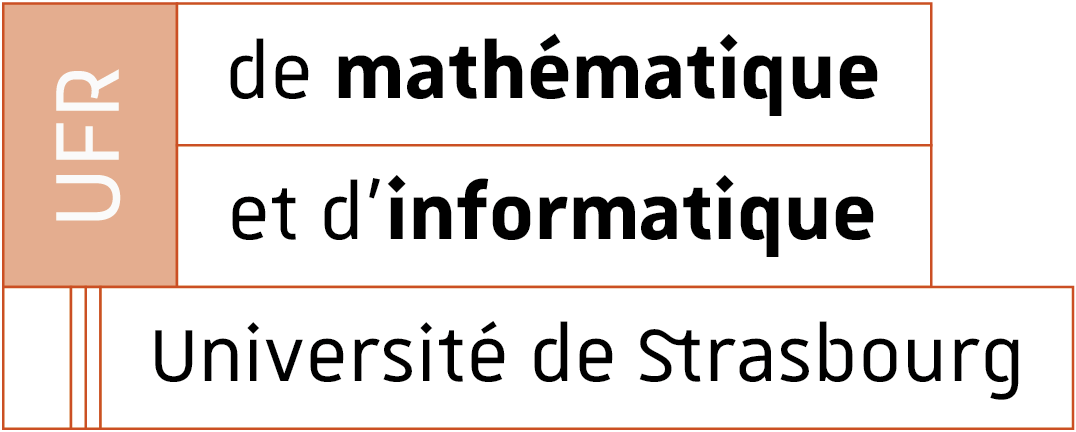
\includegraphics[width=0.5\textwidth]{images/logo_ufr.png}\par\vspace{1cm}
    \vspace{1.5cm}
    {\huge\bfseries ExaMA WP1 - Vegetation\par}
    \vspace{2cm}
    {\Large Giulio Carpi Lapi, Pierre-Antoine Senger\par}
    \vfill
    supervised by\par
    Pierre Alliez and Vincent Chabannes

    \vfill

% Bottom of the page
    {\large Date: \today\par}
\end{titlepage}

\tableofcontents
\newpage

\section{Abstract}
Urban areas are intricate systems influenced by various factors,
including vegetation, particularly trees, which play a vital role in shaping
microclimates, energy consumption, and overall livability. This project focuses
on integrating vegetation, specifically trees, into 3D geometric models of
urban environments to enhance the accuracy and realism of thermal and energy
simulations. Leveraging data from sources like OpenStreetMap, the project aims
to identify tree positions and attributes within urban landscapes and generate
a library of 3D tree models for integration into terrain meshes. Supervised by
experts from Inria and the University of Strasbourg, the project follows a
roadmap with defined milestones to deliver versions V0, V1, and V2 by specified
deadlines. Through this endeavor, the project seeks to provide valuable
insights for urban planners, architects, and policymakers, ultimately
contributing to the development of more sustainable and resilient cities.

For the \textbf{V1} version of the report add:

\begin{itemize}
    \item Methodology
    \item Results
    \item Conclusion
\end{itemize}

\newpage

\section{Introduction}
Urban areas are complex environments where various factors interact to influence 
microclimates and energy consumption. Among these factors, 
vegetation, particularly trees, plays a crucial role in shaping the urban landscape 
and its environmental characteristics. Trees provide shade, mitigate heat and can
reduce air pollution. Their strategic placement and characteristics can
significantly impact the thermal and energy dynamics of urban areas.

\begin{figure}[H]
    \centering
    \includegraphics[width=0.5\textwidth]{images/TreeShade.png}
    \captionsetup{font={scriptsize}}
    \caption{Urban trees \cite{img:TreeShade}}
\end{figure}

\begin{figure}[H]
    \centering
    \includegraphics[width=0.5\textwidth]{images/heat_street.png}
    \captionsetup{font={scriptsize}}
    \caption{Thermal image of a street in the city. \cite{img:street_thermography}}
\end{figure}

In recent years, advancements in computational modeling have facilitated the 
development of sophisticated tools for simulating the thermal and energy performance 
of urban environments. These tools rely on 3D geometric models that accurately 
represent the built environment, including buildings, roads, and terrain.

\begin{figure}[H]
    \centering
    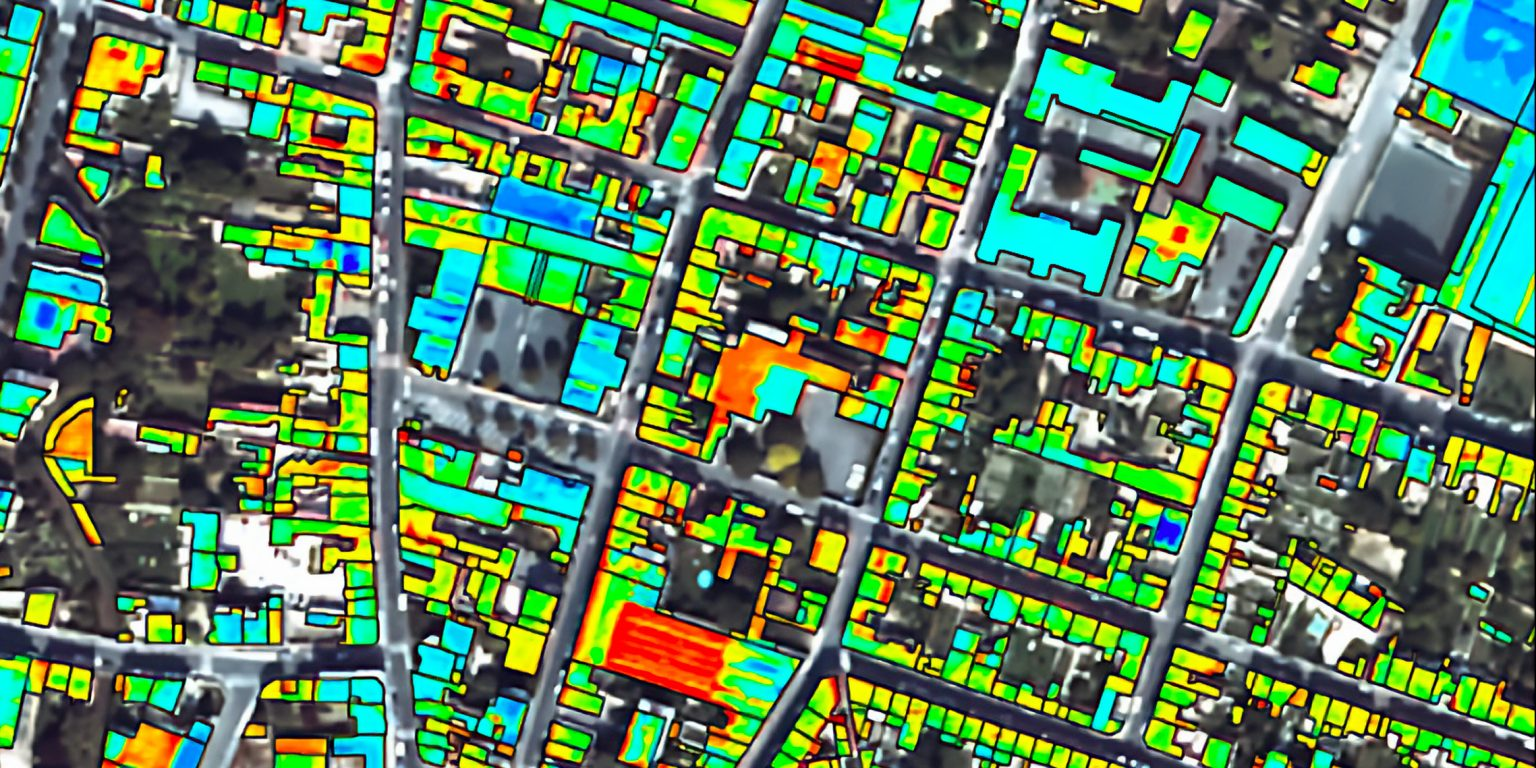
\includegraphics[width=0.5\textwidth]{images/thermographie-aerienne.jpg}
    \captionsetup{font={scriptsize}}
    \caption{Thermal image of a city \cite{img:aerialview}}
\end{figure}

The integration of vegetation into 3D urban models poses several challenges. 
Obtaining accurate data on the location, size, and species of trees within an 
urban area is non-trivial. Additionally, representing the complex geometry of trees 
in a scalable and computationally efficient manner is a significant computational 
challenge. Nevertheless, addressing these challenges is essential for creating 
realistic and reliable simulations that account for the influence of vegetation on 
urban microclimates and energy usage.

In this context, this project aims to develop a methodology for integrating 
vegetation, particularly trees, into 3D geometric models of urban areas. Leveraging 
data from sources such as the OpenStreetMap database, the project seeks to identify 
the position and attributes of trees within the urban landscape. Subsequently, a 
library of 3D tree models will be generated to accurately represent the vegetation 
in the model. Finally, these tree models will be integrated into the terrain mesh, 
enabling comprehensive simulations that consider the interactions between buildings, 
terrain, and vegetation.

By incorporating vegetation into 3D urban models, this project seeks to enhance the 
accuracy and realism of thermal and energy simulations. The resulting models will 
provide urban planners, architects, and policymakers with valuable insights into 
the environmental performance of urban areas, ultimately contributing to the 
development of more sustainable and resilient cities.

This endeavor forms a segment of a broader initiative that seeks to construct
mathematical models proficient in simulating the operations of trees within an
urban setting such as streets or parks. The project addresses pertinent
questions related to urban green spaces: optimal locations for tree placement,
the most effective arrangement strategies - whether in clusters or aligned,
and the identification of the most appropriate methods to generate the coolest
possible climatic conditions.

The project is supervised by Pierre Alliez
Senior Researcher at Inria center at Côte d'Azur University
and by Vincent Chabannes research engeneer at the University of Strasbourg.
We will have weekly meetings with them to discuss the progress of the project.
The deadlines we have set are the following:
\begin{itemize}
    \item \textbf{V0} : due by March 26, 2024
    \item \textbf{V1} : due by April 23, 2024
    \item \textbf{V2 - Final} : due by May 28, 2024
\end{itemize}

With the help of our supervisors, we have defined the following roadmap:

\begin{figure}[H]
    \centering
    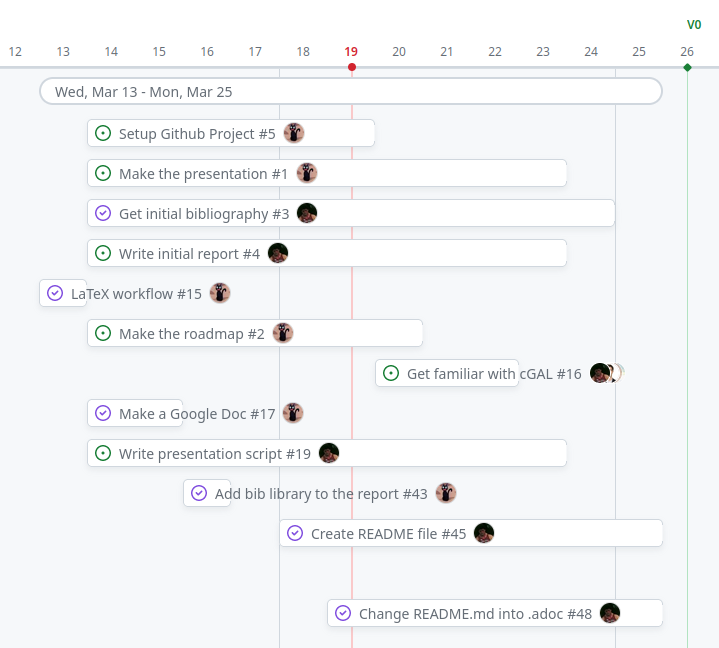
\includegraphics[width=0.5\textwidth]{images/roadmap_v0.png}
    \captionsetup{font={scriptsize}}
    \caption{Roadmap v0}
\end{figure}

\begin{figure}[H]
    \centering
    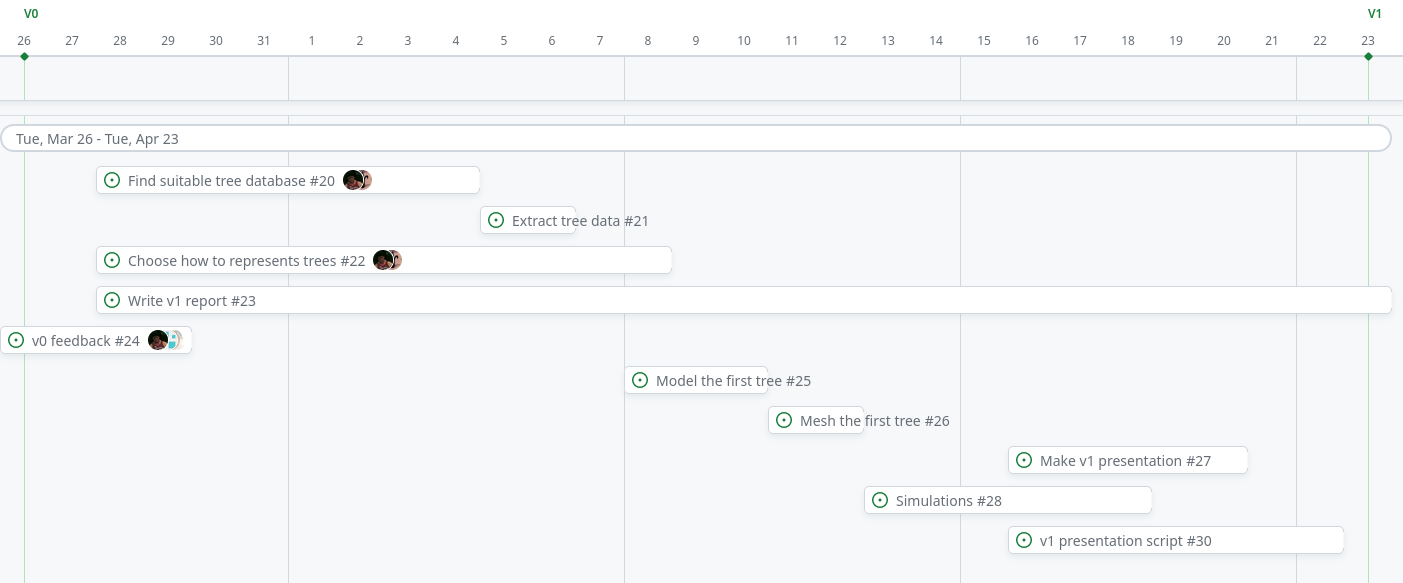
\includegraphics[width=0.5\textwidth]{images/roadmap_v1.png}
    \captionsetup{font={scriptsize}}
    \caption{Roadmap v1}
\end{figure}

\begin{figure}[H]
    \centering
    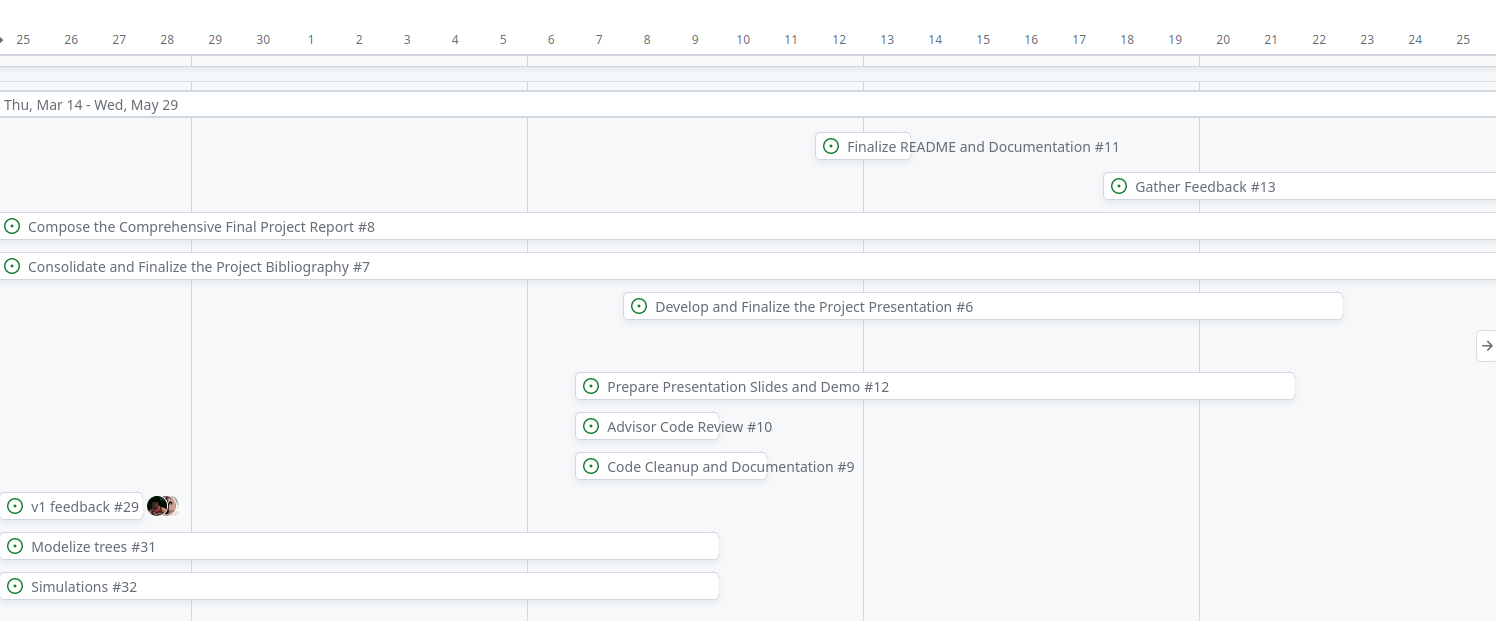
\includegraphics[width=0.5\textwidth]{images/roadmap_v2.png}
    \captionsetup{font={scriptsize}}
    \caption{Roadmap v2}
\end{figure}

This will help us to keep track of the progress of the project and to make sure
we are going to deliever the respective versions on time.

This project will be developed in C++.
For the geometric aspect of tree model and meshing we will use the CGAL library.
CGAL is an open source software project that provides easy access to efficient
and reliable geometric algorithms in the form of a C++ library which is used
in various areas needing geometric computation.\cite{cgal}

\begin{figure}[H]
    \vspace{1.5cm}
    \centering
    \includegraphics[width=0.5\textwidth]{images/cgal_logo.png}
\end{figure}

Softwares like MeshLab, an open source system for processing and editing 3D
triangular meshes\cite{meshlab}, will allow us to visualize the 3D models trees generated with
the help of CGAL.

We will be working with different Levels of Detail (LOD) for the 3D models.
Starting with LOD0, which represents the least detailed version of the model,
we will progressively complexify the model to LOD1 and LOD2.
Each level adds complexity to the model, making it more
resource-intensive to render.



\begin{figure}[H]
    \vspace{1.5cm}
    \centering
    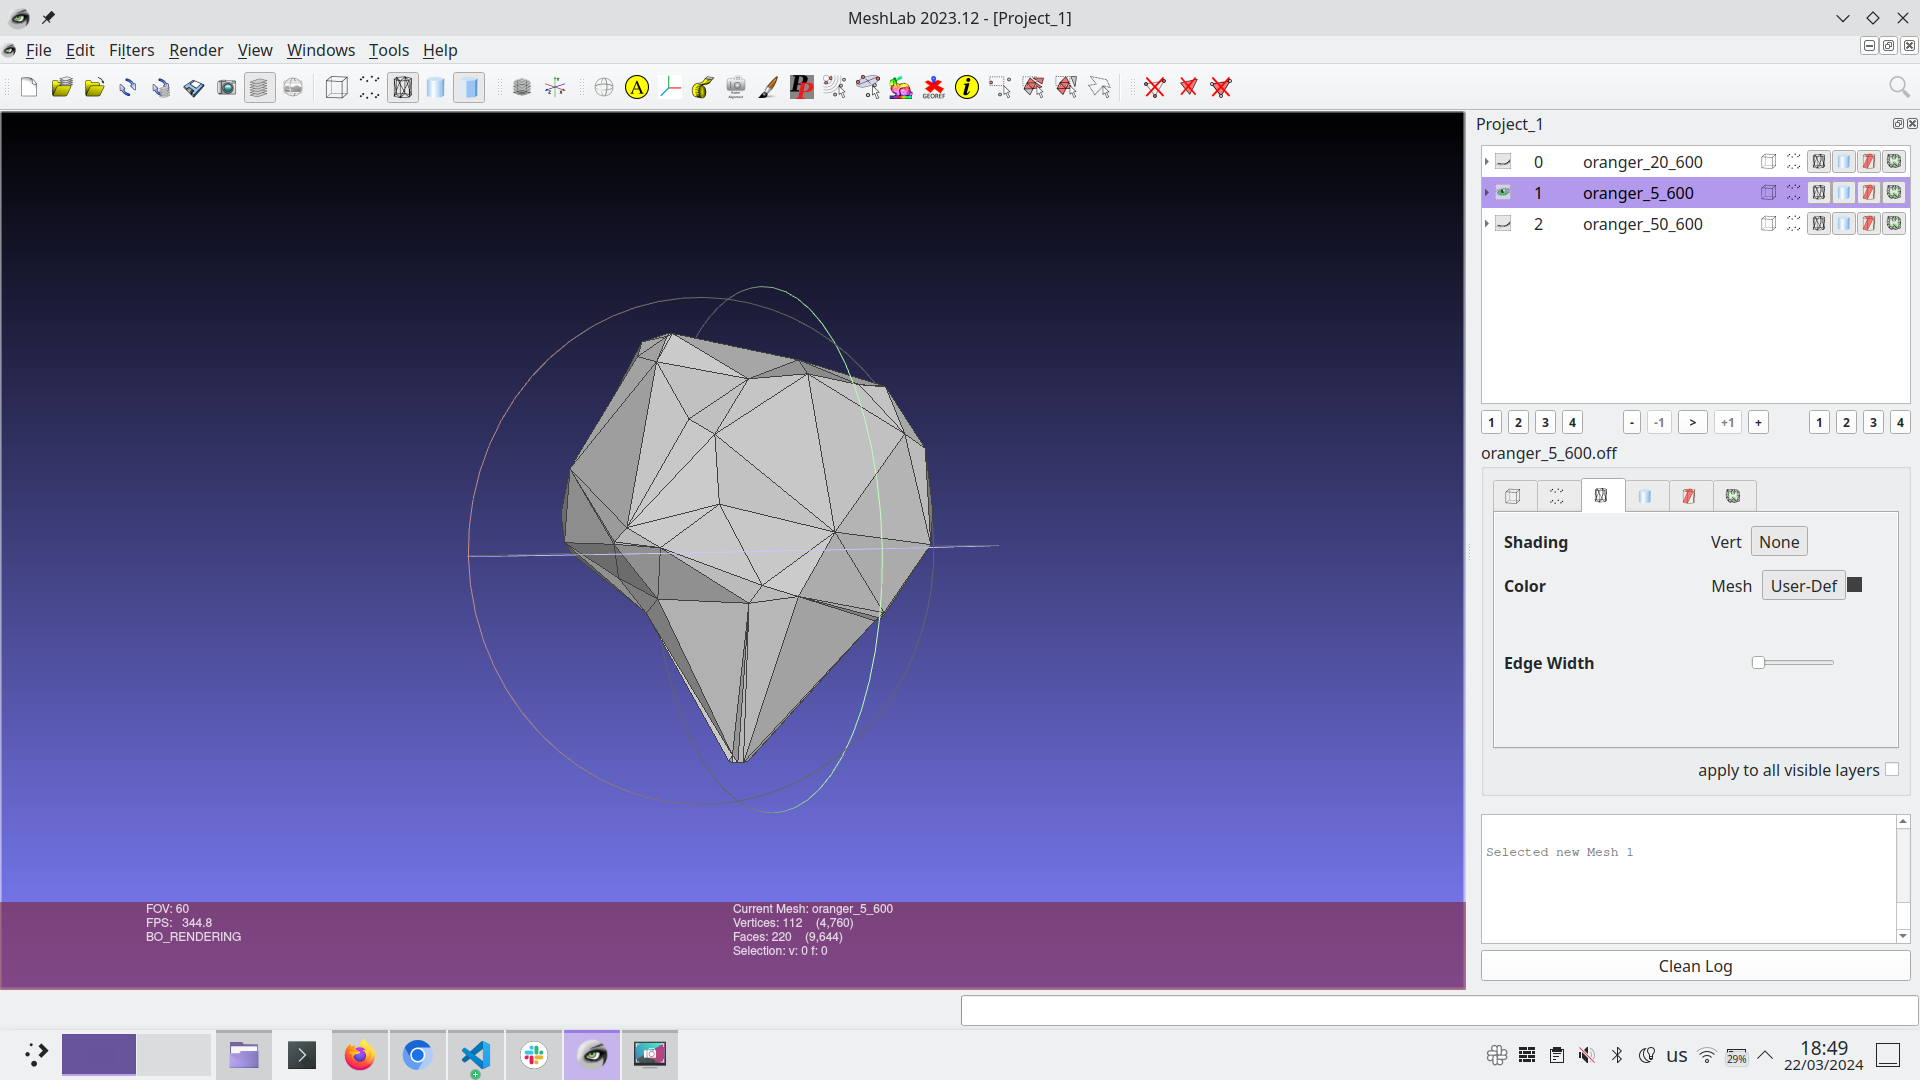
\includegraphics[width=0.5\textwidth]{images/LOD0.png}
    \captionsetup{font={scriptsize}}
    \caption{LOD0}
\end{figure}

\begin{figure}[H]
    \vspace{1.5cm}
    \centering
    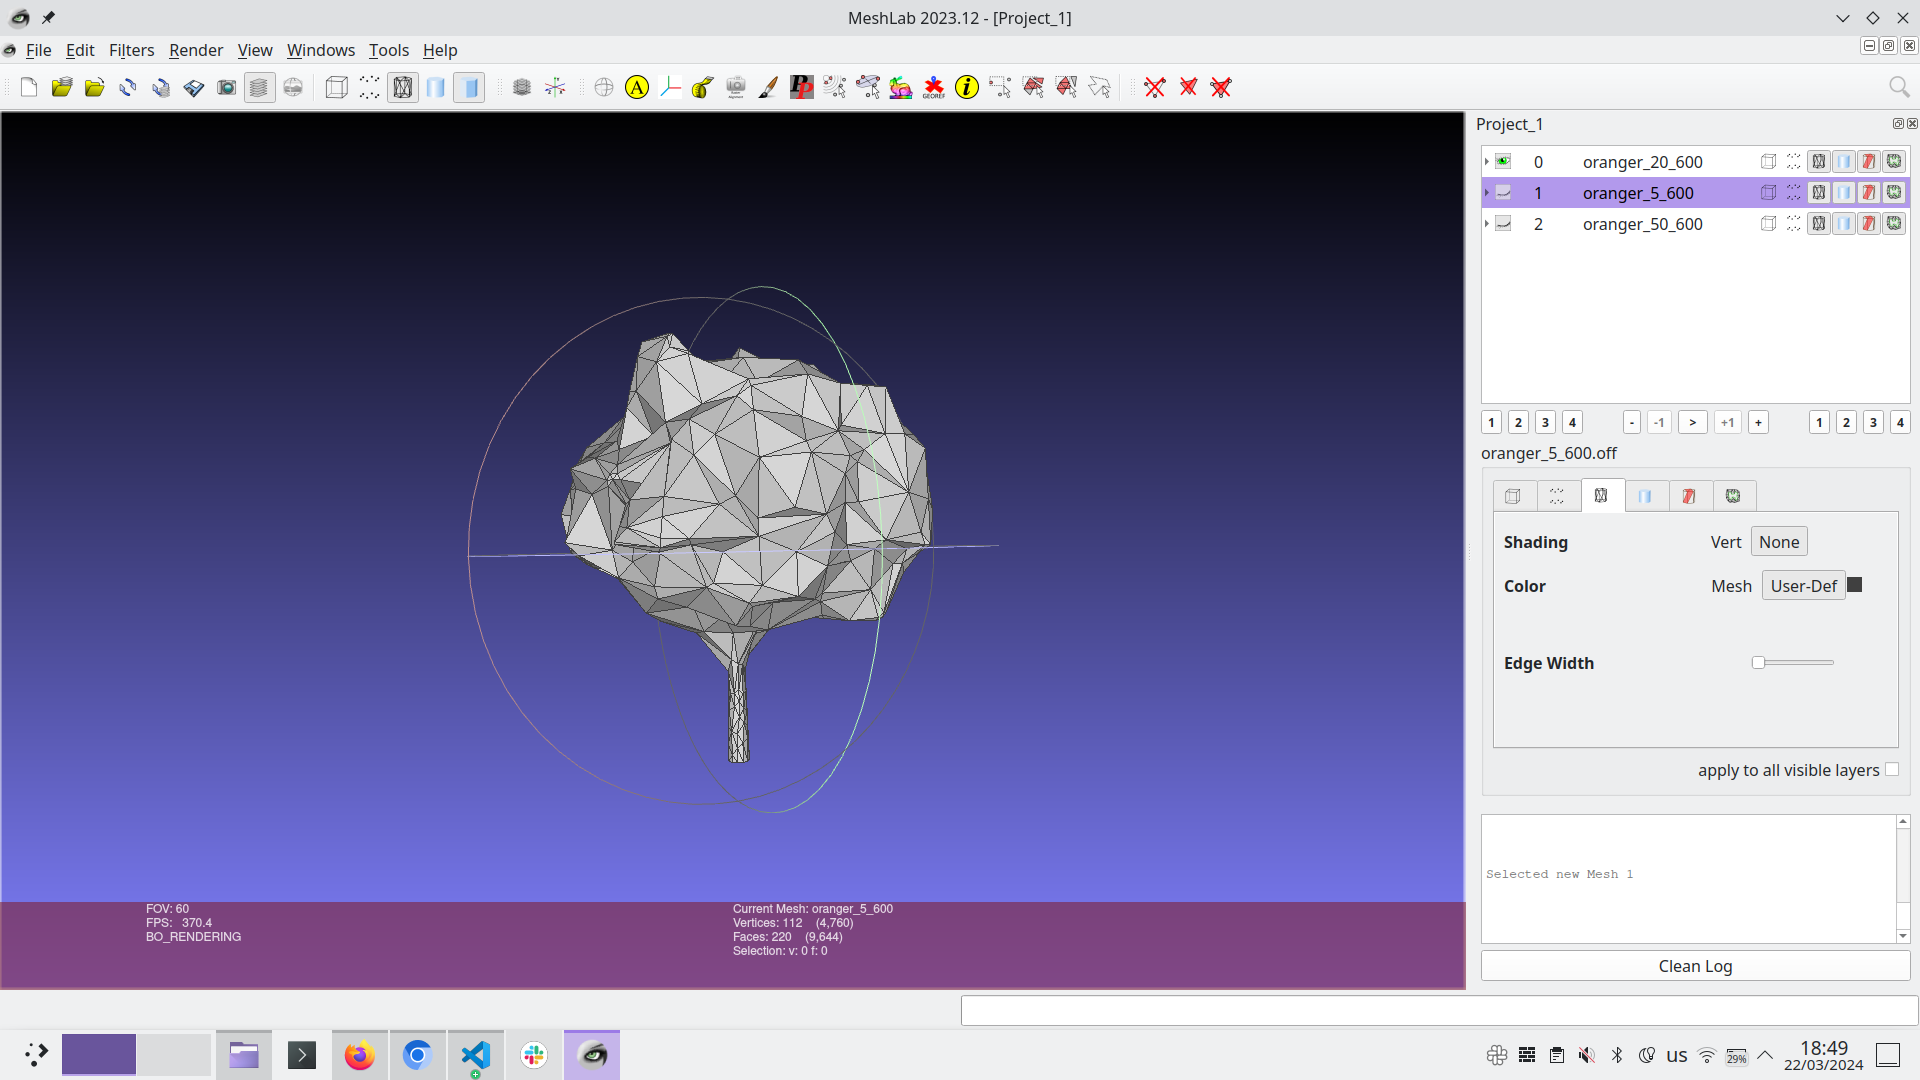
\includegraphics[width=0.5\textwidth]{images/LOD1.png}
    \captionsetup{font={scriptsize}}
    \caption{LOD1}
\end{figure}

\begin{figure}[H]
    \vspace{1.5cm}
    \centering
    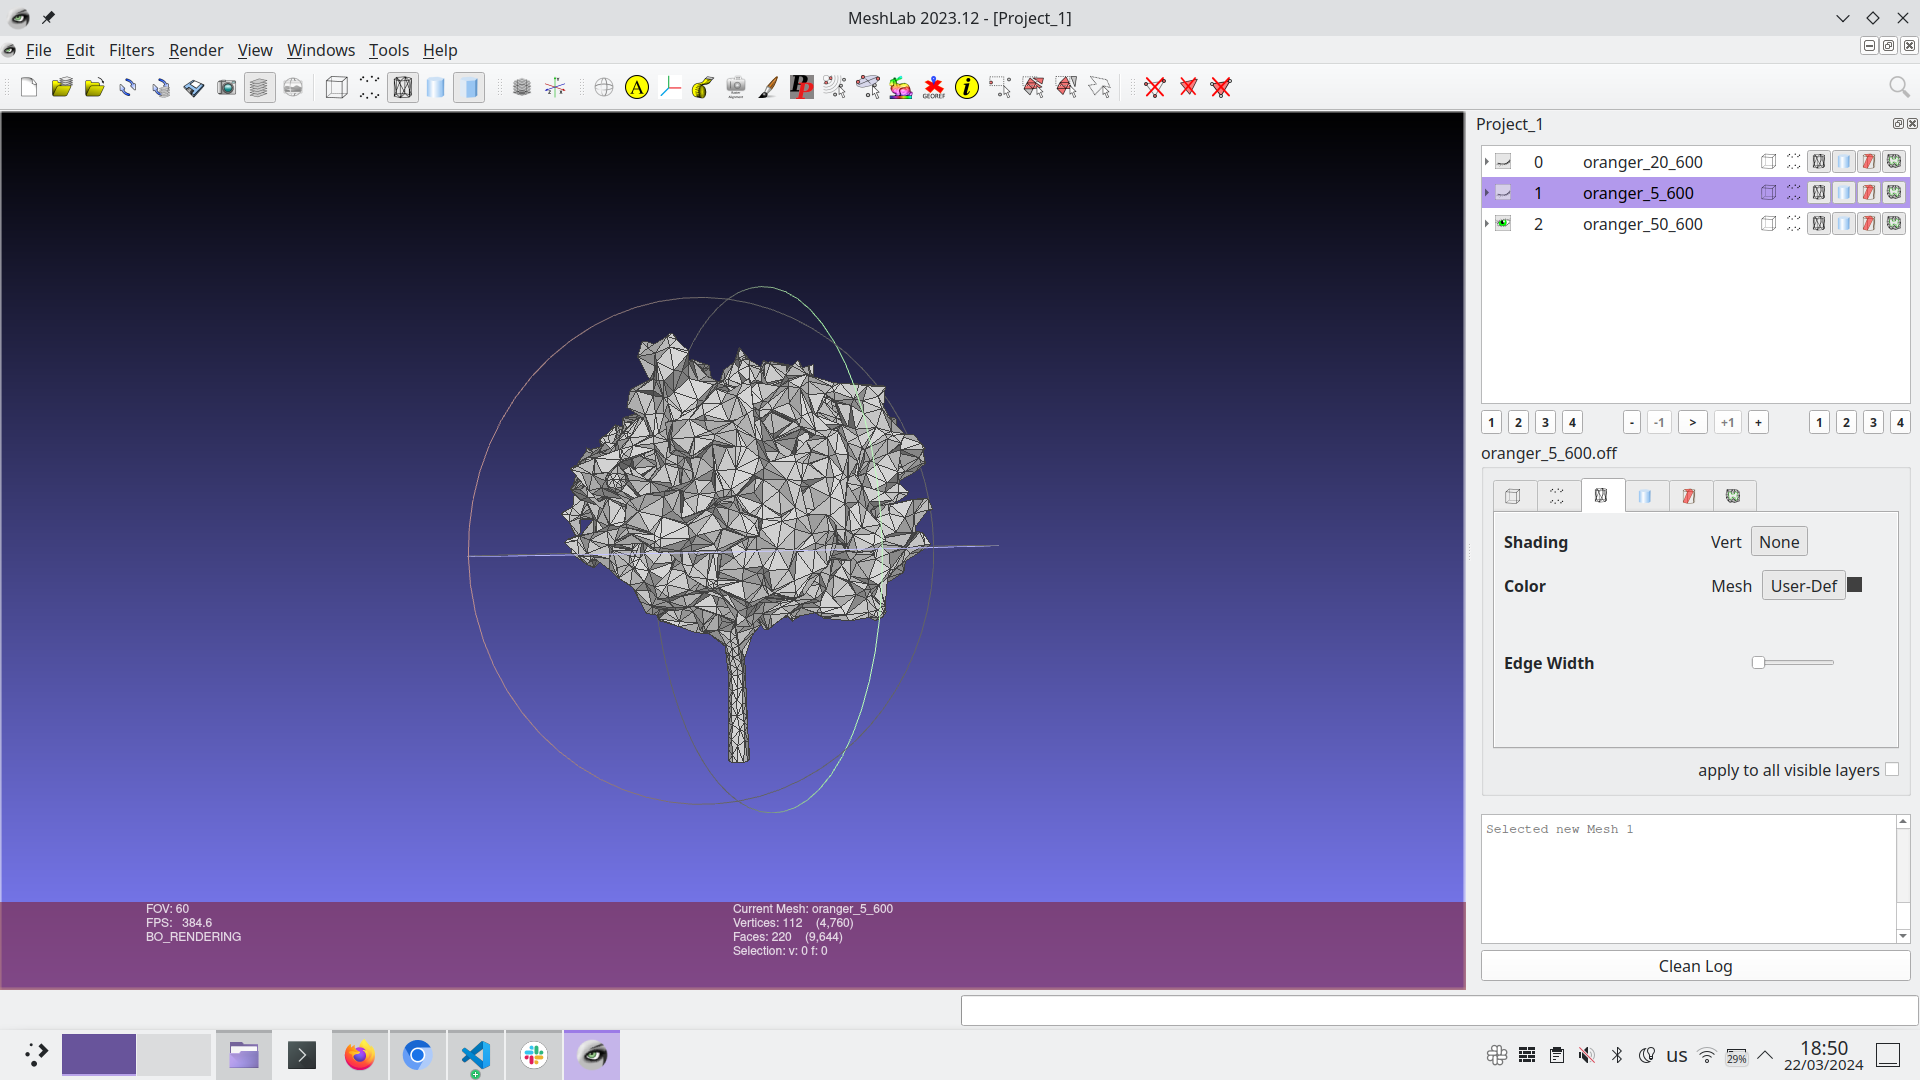
\includegraphics[width=0.5\textwidth]{images/LOD2.png}
    \captionsetup{font={scriptsize}}
    \caption{LOD2}
\end{figure}

We will be using the Feel++, an open-source C++ library, to calculate the
shading on buildings. This library is particularly suited for solving
Partial Differential Equations (PDEs), which are essential in the computation
of light and shade on 3D objects\cite{feel++}. By leveraging the capabilities of Feel++,
we can accurately simulate the shading effects on our LOD models of buildings.

\newpage
\section{Literature Review}

\newpage

\section{Methodology}

\newpage

\section{Results}

\newpage

\section{Conclusion}

\newpage

\section{References}
\nocite{*}
\bibliographystyle{plain}
\bibliography{references}

\end{document}